\chapter{Results}
\label{sec:results}
In previous chapters, different methods were introduced that are available for selected use cases in biology and medicine research. 
%\section{Virtual Infrastructure}
%\label{sec:resultsinfrastructure}
As each of the use cases and available systems were proposed on different operating system platforms, architecture and/or middleware, the virtualization was utilized to build the virtual infrastructure for the purposes of each pilot application. The paper \cite{kulhanek2010c} \emph{Infrastructure for Data Storage and Computation in Biomedical Research} in Appendix~\ref{app:infrastructure} describes the result of establishing virtualization on a physical infrastructure in order to share computational power among different platforms.

\section{Medical Images}
\label{sec:resultsimages}

%Within the virtual infrastructure, the pilot grid infrastructure was established in the location of First Faculty of Medicine, Charles University in Prague, Central Military Hospital in Prague and CESNET association. And the Globus Toolkit middleware and Globus MEDICUS implementation was installed on linux based virtual machines using XEN hypervisor providing pilot services to access this grid based PACS system.

The pilot infrastructure of several servers was installed in several institutions in Prague, Czech Republic. Globus Toolkit and Globus MEDICUS were installed on them. The paper \cite{kulhanek2009}  \emph{Processing of Medical Images in Virtual Distributed Environment}, in Appendix~\ref{app:processing}, published details about the integration of Globus MEDICUS with a MeDiMed project. It concludes that such integration via the DICOM protocol is almost seamless. Furthermore, if such a grid-based system is joined with a production system for exchanging clinical DICOM data, it could be beneficial for researchers.

\section{Remote Access To Voice Analysis}
\label{sec:resultsvoice}

The paper \cite{kulhanek2010b} \emph{Remote Analysis of Human Voice--Lossless Sound Recording Redirection}, in the Appendix~\ref{app:remote}, published technical details and results of customizing a RDP protocol for lossless sound recording redirection. It also discusses remote access via a remote desktop feature of Windows platform to an application in order to analyze human voice and produce a voice range profile for further use. 

Additionally, the 
%custom RDP plugin with the ParVRP and RealVoiceLab software to redirect the sound recording without loss of information 
remote application
was packaged as a virtual machine template. This was deployed in the pilot virtual infrastructure next to the test instance of Globus MEDICUS. The virtual machine template was also deployed to different cloud computing infrastructures. The first was deployed to the Amazon EC2\footnote{\url{http://aws.amazon.com/ec2/} accessed February 2015} and the second to the pilot scientific cloud, MetaCloud\footnote{\url{http://www.metacentrum.cz/en/cloud/} accessed February 2015}. In the EGI Technical Forum 2012, such comparison was presented to the user and technical community within CESNET and EGI organization\cite{Kulhanek2012a}.

\section{Parameter Estimation}
\label{sec:resultsestimation}

The paper \cite{Kulhanek2014Parameters} \emph{Parameter Estimation of Complex Mathematical Models of Human Physiology Using Remote Simulation Distributed in Scientific Cloud}, in Appendix~\ref{app:parameter}, published the architecture and measurement of a speedup that was achieved on estimating parameters of three different types of models - from the non-complex, medium-complex and complex models. It concluded that only medium-complex and complex models may benefit from the architecture as the communication overhead may become major for simple models and decrease the overall performance. 

Additionally, a scientific result was published in the paper \cite{Matejak2014sj} \emph{Adair-based Hemoglobin Equilibrium with Oxygen, Carbon Dioxide and Hydrogen Ion Activity}, in Appendix~\ref{app:adair}, where a mathematical model of hemoglobin integrating \ce{O_2}, \ce{CO_2} and \ce{H^+} binding based on theoretical principles, which were verified on the parameter estimation algorithm system\cite{Kulhanek2014Parameters}, together with methods available in Wolfram \emph{MATHEMATICA} 9.0\footnote{\url{http://www.wolfram.com/mathematica/}accessed February 2015}.

Thus, the overall performance and speedup estimation were tested against the Modelica implementation of complex physiological model HumMod \cite{Kofranek2011hummod}; the Modelica implementation of a model of hemodynamics of the cardiovascular system, published by Meurs \cite{Meurs2011}; the model of binding gases to hemoglobin, published by Matejak \cite{Matejak2014sj} and the trivial model of a curve $f(x)$ with four parameters $a,b,c,d$ defined as $ f(x)=a\cdot sin(b\cdot (x-c))+x\cdot d$ and named as "SinusCurve".
%corrections April 2nd
\sisetup{round-mode=figures,round-precision = 4}
\begin{table}[htb]
\footnotesize
\begin{tabular}{|l|r|r|r|r|r|r|r|}
\hline
complexity & name & $T_{1~[s]}$ & $T_{2~[s]}$ & $T_{3~[s]}$ & $T_{4~[s]}$ & $\alpha$ & $S$ \\
\hline
high & HumMod \cite{Kofranek2011hummod} & $\num{4639}$ & $\num{4639}$ & $\num{4618}$ & $\num{4616}$ & $\num{8.85837717978788E-005}$ & $\num{11288.7493917249}$ \\
medium & Meurs2011\cite{Meurs2011} & $\num{661.817}$ & $\num{661.490}$ & $\num{634.694}$ & $\num{634.457}$ & $\num{0.0004940943}$ & $\num{2023.9051987766}$ \\
low & Matejak2014\cite{Matejak2014sj} & $\num{17.868}$ & $\num{17.610}$ & $\num{1.399}$ & $\num{1.123}$ & $\num{0.014439221}$ & $\num{69.2558139535}$ \\
trivial & SinusCurve & $0.073$ & $0.020$ & x & x &  $\num{0.7260273973}$ & $\num{1.3773584906}$\\
\hline
\end{tabular}
\caption{Time spent in different parts of the parameter estimation algorithm for one processor deployment utilizing virtual machine on physical hardware 2x 6-core Intel E5-2620 2GHz. Genetic algorithm works with a population of $120$ individuals for $10$ generations. T1 -- is the whole time of the computation, T2 -- is the time of the computation, which can be parallelized, T3 -- time spent within the worker node, T4 -- time spent in simulation, $\alpha$ -- computed as $1-(T2/T1)$ and $S$ is the theoretical speedup limit per Amdahl's law ($1/\alpha$) eq.(\ref{eq:amdahl}).}
\label{table:speedupresult}
\end{table}

\begin{table}[htb]
\footnotesize
\begin{tabular}{|l|r|r|r|r|r|r|r|}
\hline
complexity & name & $T_{1~[s]}$ & $T_{2~[s]}$ & $T_{3~[s]}$ & $T_{4~[s]}$ & $\alpha$ & $S$ \\
\hline
high & HumMod \cite{Kofranek2011hummod} & $\num{6463.217}$ & $\num{6460.937}$ & $\num{6451.079}$ & $\num{6458.253}$ & $\num{0.000352766}$ & $\num{2834.744}$ \\
medium & Meurs2011\cite{Meurs2011} & $\num{699.631}$ & $\num{699.228}$ & $\num{697.907}$ & $\num{696.948}$ & $\num{0.000576018}$ & $\num{1736.057072}$ \\
low & Matejak2014\cite{Matejak2014sj} & $\num{2.893}$ & $\num{2.373}$ & $\num{1.228}$ & $\num{1.149}$ & $\num{0.17974421}$ & $\num{5.563461538}$\\ \hline
\end{tabular}
\caption{Same as Table \ref{table:speedupresult}, but measured on a local server deployment, with reduced communication overhead.}
\label{table:speedupresult2}
\end{table}

The computation time of a single simulation depends mainly on the model complexity. Based on the findings, the simulations of the models were divided into four groups, depending on its demand to compute $\num{1200}$ simulations. Speedup is studied for these four groups and Amdahl's law is appropriate to estimate upper limit of it as discussed in Section \ref{sec:parallelprogramming}. Fraction $\alpha$ and the speedup limit per Amdahl's law are stated in Tables \ref{table:speedupresult} and \ref{table:speedupresult2}. 

The difference between $T_2$ and $T_3$ is an overhead, which was introduced by the network communication between the genetic algorithm and the worker nodes that were deployed in the cloud deployment, provided by CESNET NGI department METACENTRUM\footnote{\url{http://www.metacentrum.cz} accessed March 2015}. The network overhead can be eliminated in serial implementations by directly integrating the simulation into a genetic algorithm. Therefore, Table \ref{table:overhead} considers and compares a hypothetical serial execution time, which is estimated without the network overhead.

\begin{table}[ht]
\footnotesize
\begin{tabular}{|l|r|r|r|r|r|r|r|r|}
\hline
& \multicolumn{4}{c|}{distributed in cloud} & \multicolumn{4}{c|}{distributed in local cluster} \\
 & \multicolumn{2}{c|}{overhead} & \multicolumn{2}{c|}{est. serial} & \multicolumn{2}{c|}{overhead} & \multicolumn{2}{c|}{est. serial} \\
model name & $T_2-T_{3~[s]}$ & fraction$_{[\%]}$ & $T_{es~[s]}$ & $S_{es}$ & $T_2-T_{3~[s]}$ & fraction$_{[\%]}$ & $T_{es~[s]}$ & $S_{es}$\\
\hline
HumMod \cite{Kofranek2011hummod} & $\num{20.983}$ & $\num{0.45225141}$ & $\num{4618.693}$ & $\num{1.0045430601}$ & $\num{9.858}$ & $\num{0.15252466}$ & $\num{6453.359}$ & $\num{1.0015275766}$ \\
Meurs2011 \cite{Meurs2011} & $\num{26.796}$ & $\num{4.04885338}$ & $\num{635.021}$ & $\num{1.0421970297}$ & $\num{1.321}$ &  $\num{0.18881382}$ & $\num{698.310}$ &$\num{1.00189171}$\\
Matejak2014\cite{Matejak2014sj} & $\num{16.211}$ & $\num{90.72643833}$ & $\num{1.657}$ & $\num{10.7833433917}$ & $\num{1.145}$ &  $\num{39.57829243}$ & $\num{1.748}$ &$\num{1.6550343249}$\\
\hline
\end{tabular}
\caption{ Comparison in cloud deployment vs. local cluster deployment of communication overhead. Its fraction in the whole computation was introduced by the network transfer speed and latency. The estimated time and speedup, if the worker is replaced by a serial version of computation without communication overhead, is: $T_{es}$ -- estimated time of serial version of computation. $S_{es}$ -- estimated speedup of serial version of computation against the parallel on one processor.}
\label{table:overhead}
\end{table}

The speedup was measured on 10 CPUs till 60 CPUs and compared in order to predicted the speedup, as seen in Figure \ref{fig:amdahlres}. Similar  measurements with different parameters of genetic algorithm were carried out using 80 and 160 CPUs, as seen in Table \ref{table:speedupresult3}.

\begin{table}[htb]
\footnotesize
\begin{tabular}{|l|r|r|r|r|r|}
\hline
complexity & name & $T_1(80)_{[s]}$ & $S(80)$ & $T_1(160)_{[s]}$ & $S(160)$\\
\hline
high & HumMod \cite{Kofranek2011hummod} & $\num{544.539}$ & $\num{63.9807249802}$ & $\num{286.657}$ & $\num{121.5389821285}$ \\
medium & Meurs2011\cite{Meurs2011} & $\num{90.991}$ & $\num{55.9311360464}$ & $\num{96.000}$ & $\num{53.0128125}$ \\
low & Matejak2014\cite{Matejak2014sj} & $\num{11.378}$ & $\num{16.6865881526}$ & $\num{15.128}$ & $\num{12.5500720509}$\\ \hline
\end{tabular}
\caption{Scalability on 80 CPUs and 160 CPUs of parameter estimation on cloud computing cluster on 5-10 virtual machines, each 16 CPUs on physical hardware 2x 8-core Intel E5-2670 2.6GHz. Genetic algorithm configured with a population $640$ individuals for $20$ generations, which increases about 10 times more simulation performed compared to previous tables. Speedup estimated from measuring the computation when using 1 CPU.}
\label{table:speedupresult3}
\end{table}

\begin{figure}[htb]
    \centering
    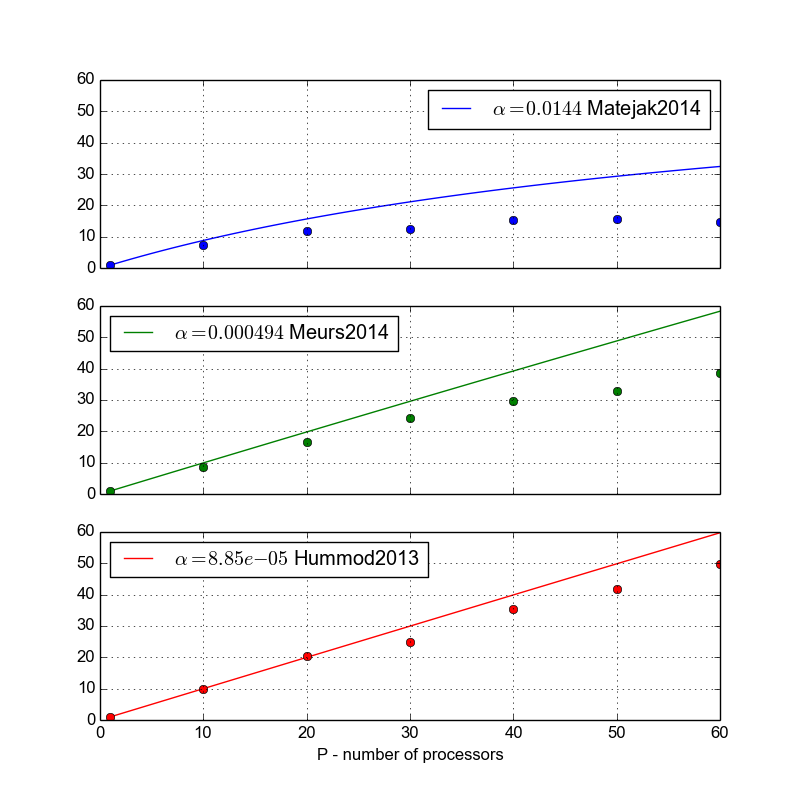
\includegraphics[width=0.9\textwidth]{chapter7/speedup.png}
    \caption{Estimated speedup (lines) per Amdahl's law (eq.\ref{eq:amdahl} \cite{Amdahl1967}) for different $\alpha$ of several Modelica models and real measured speedup (points) on cloud deployed on 1-6 virtual machines on physical hardware (2x 6-core Intel E5-2620 2GHz, 1Gbit/s Ethernet.)  }
    \label{fig:amdahlres}
\end{figure}

To summarize the results from Table \ref{table:speedupresult3} and Figure \ref{fig:amdahlres}, the low complex model scales up to 40 CPUs with a speedup of 15 (compare to theoretical serial speedup of 11, if eliminating network overhead,  Table \ref{table:overhead}). The medium complex model scales up to 80 CPUs with a speedup of 56 and complex model scales up to 160 CPUs (and probably more) with a speedup of 122. Practically, good parameter estimation was obtained after 200 generations with population of 640, which implicates that the computation time can be reduced from four days to 47 minutes in the case of complex model and from 14 hours to 15 minutes in the case of medium complex model.
%40 proc 15, 80 proc 56, 160 proc 121,our dYA TO47 from 17 hours to 18minnutes

The deployment on local cluster reduces the communication overhead. However, in order to compute concurrently, it is limited by available processors. Thus, computing on local cluster should be considered for boundary cases like the simple models. The following statement can be made:
\begin{itemize}
\item{If the alpha fraction is major, then a serial computation of parameter estimation algorithm without communication overhead, will perform best. This is the case for the trivial function. }
\item{If the alpha fraction is minor, but the network overhead is still major a computation on local cluster or virtual HPC cluster should be considered. This is the case for the low complex model simulation, e.g.  Matejak2014\cite{Matejak2014sj}.} 
\item{If the alpha fraction is minor and the network overhead is also minor, then the distributed computation, e.g., in a cloud-computing environment, is worth using. This is the case of the medium and high complex model simulations of "Meurs2011" \cite{Meurs2011} and "HumMod2013" \cite{Kofranek2011hummod}.}
\end{itemize}

\begin{figure}[htb]
    \centering
    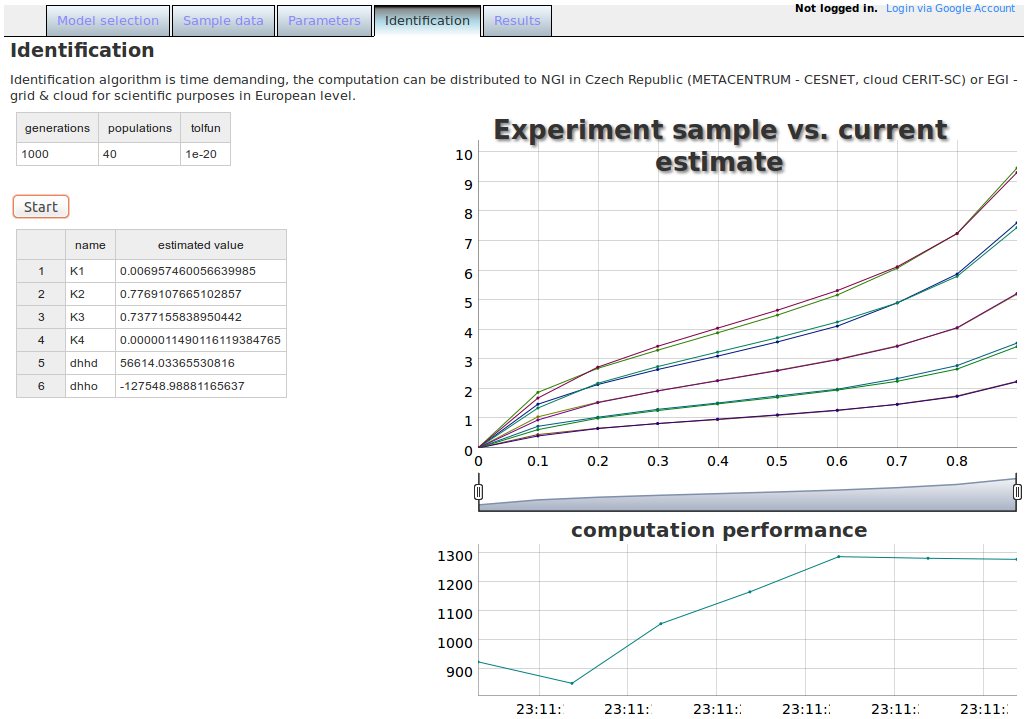
\includegraphics[width=1\textwidth]{chapter7/app-physiovalues.png}
    \caption{User interface of a web application for parameter estimation. In this case, for the model Matejak2014\cite{Matejak2014sj}. The top left table lists the parameters for the genetic algorithm($\num{1000}$ generations with a population size of $40$ and a cumulative change in the generation limit, which ends the algorithm earlier). The middle left table shows the model parameters and current best values, which fit the sample data. The chart shows how the sample data fits with the model simulation. The right bottom chart shows the performance of computation in a number of model simulations per second.}
    \label{fig:app.physiovalues}
\end{figure}

\subsection{Parameter Sweep}
\label{sec:resultsboinc}
The desktop grid BOINC system was established for parameter sweep application. The established project, \emph{Physiome@home}, and it's project web page, \url{http://physiome.lf1.cuni.cz/ident3/physiome}, manages workunit tasks which are sent to and executed by BOINC workers. The worker application is a packaged model that is exported as FMU for a Windows platform and wrapper application, which communicates with the BOINC manager on the desired volunteer computer. 

%This project is now  distribute computational tasks into computers in scholar labs, which may in iddle time contribute to the computing demands. Because BOINC is very popular and users joins to a teams to compete with several types of competition, this particular project attracts after 2 weeks 78 participants from all around the world. 


\subsection{Remote Simulation and Local Visualization}
An extra outcome of an architecture for parameter estimation is a hybrid web simulator system, where a single instance of a worker node is utilized as a back-end for the simulation engine. The front-end presented as a web application, is implemented using HTML and Javascript libraries in order to visualizes and control the simulation on the worker, as seen in Figure \ref{fig:sim.physiovalues}.
The results were published in \cite{Kulhanek2013c} and popularized in \cite{Kulhanek2013b}.

\begin{figure}[htb]
    \centering
    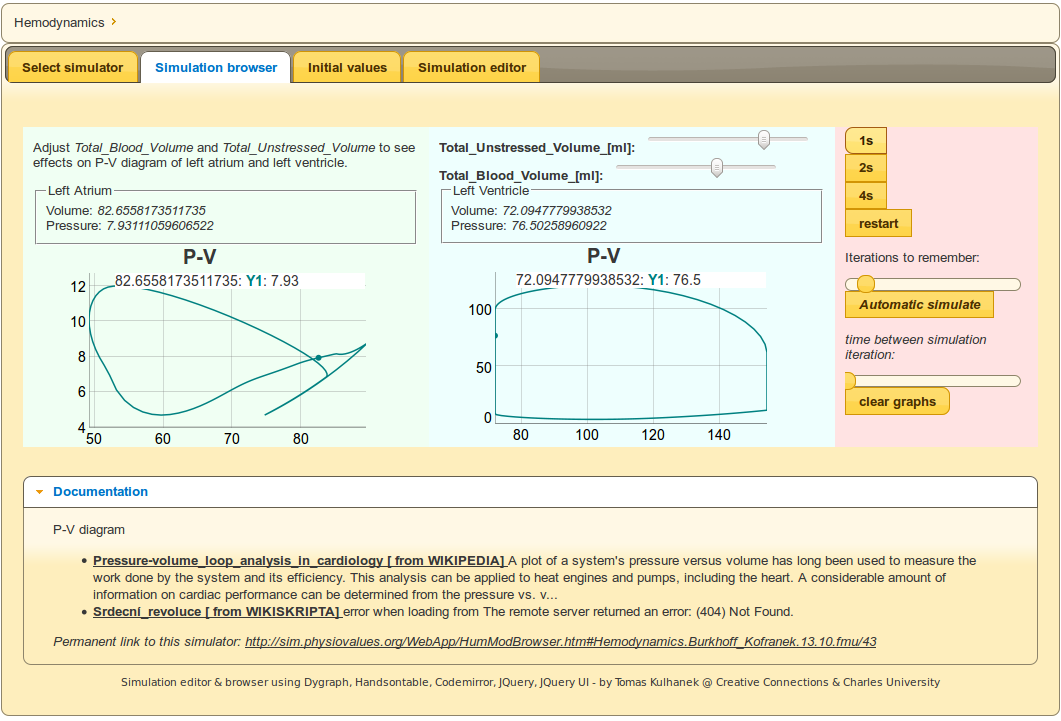
\includegraphics[width=1\textwidth]{chapter7/sim-physiovalues.png}
    \caption{Web application to visualize simulation, in this case, pressure volume diagrams of the left atrium and left ventricle of the model of hemodynamics of a cardiovascular system.}
    \label{fig:sim.physiovalues}
\end{figure}

\subsection{Summary}

A pilot web domain was established to include the previous results and to start collecting the physiological relevant values at \url{http://www.physiovalues.org}. 
Further development may focus on connecting values of parameters and variables with a physiological or pathological scenario. 